\documentclass{beamer}

\usecolortheme[light]{solarized}

\beamertemplatenavigationsymbolsempty

\usepackage{hyperref}
\usepackage{minted}

\usepackage{graphicx}
\usepackage{tikz}

\usetikzlibrary{calc, patterns}

\begin{document}

    \begin{frame}
        \begin{center}
            \Large

            Redesigning a course to include research led teaching (using
            software development methodologies)\pause (so as to encourage an
            active learning environment) \pause (using a flipped learning
            approach) \pause (... open teaching resources ...) \pause
            (... sustainable software fellow ...)\pause (and some other stuff)

        \end{center}
    \end{frame}

    \begin{frame}
        \small
        \begin{quote}
            `In the STEM classroom should we ask or should we tell?''
        \end{quote}

        \begin{center}
            \textbf{Active learning increases student performance in
            science, engineering, and mathematics} Freeman et al. 2014 (PNAS)
        \end{center}
    \end{frame}


    \begin{frame}
		\begin{center}
            \frame{\includegraphics[height=.8\textheight]{./static/flipped_learning.jpg}}
		\end{center}
	\end{frame}

    \begin{frame}
        \Huge
        \begin{center}
            Video
        \end{center}
    \end{frame}

    \begin{frame}
		\begin{center}
			\includegraphics[width=.6\textwidth]{./static/time_for_this_again.png}
		\end{center}
	\end{frame}

    \begin{frame}
		\begin{center}
            \includegraphics[width=.8\textwidth]{./static/scaffolding_vs_pedagogic_premise.pdf}
		\end{center}
	\end{frame}

    \begin{frame}
        \begin{center}
			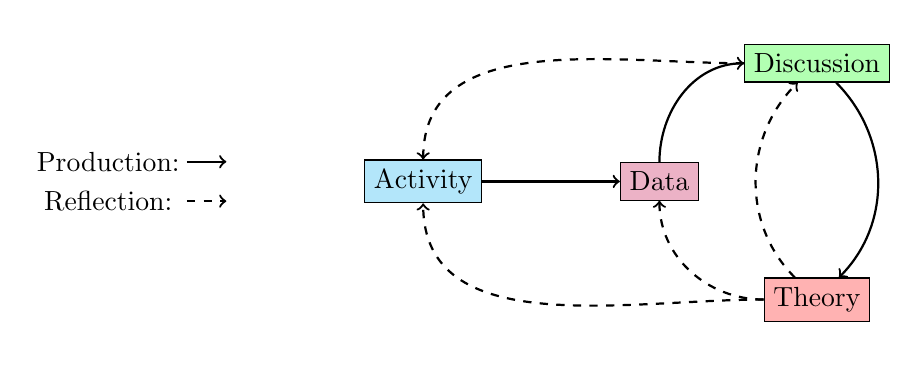
\begin{tikzpicture}
				% Nodes
				\node (activity) at (0,0) [fill=cyan!30, draw] {Activity};
				\node (data) at ($(activity) + (3,0)$) [fill=purple!30, draw] {Data};
				\node (discussion) at ($(data) + (2,1.5)$) [fill=green!30, draw] {Discussion};
				\node (theory) at ($(data) + (2,-1.5)$) [fill=red!30, draw] {Theory};

				% Creative arrows
				\draw [thick, ->] (activity) -- (data);
				\draw [thick, ->] (data) edge[out=90, in=180] (discussion);
				\draw [thick, ->] (discussion) edge[out=-45, in=45] (theory);

				% Reflective arrows
				\draw [thick, ->, dashed] (theory) edge[out=180, in=-90] (data);
				\draw [thick, ->, dashed] (theory) edge[out=180, in=-90] (activity);
				\draw [thick, ->, dashed] (discussion) edge[out=180, in=90] (activity);
				\draw [thick, ->, dashed] (theory) edge[out=135, in=-135] (discussion);

				% Key
				\draw [thick, ->] ($(activity) + (-3,.25)$) -- ($(activity) + (-2.5,.25)$);
				\node at ($(activity) + (-4, .25)$) {Production:};
				\draw [thick, ->, dashed] ($(activity) + (-3,-.25)$) -- ($(activity) +
				(-2.5,-.25)$);
				\node at ($(activity) + (-4, -.25)$) {Reflection:};

			\end{tikzpicture}
        \end{center}

        \begin{center}
            \textbf{Playing Games: A Case Study in Active Learning Applied to Game Theory} Knight. 2015 (MSOR Connections)
        \end{center}
	\end{frame}

    \begin{frame}
        \begin{center}
            \includegraphics[width=.8\textwidth]{./static/white_board.jpg}
        \end{center}
    \end{frame}


	\begin{frame}
		\begin{center}
            \includegraphics[width=.6\textwidth]{./static/ssi-logo.png}
        \end{center}
	\end{frame}

    \begin{frame}
        \begin{center}
            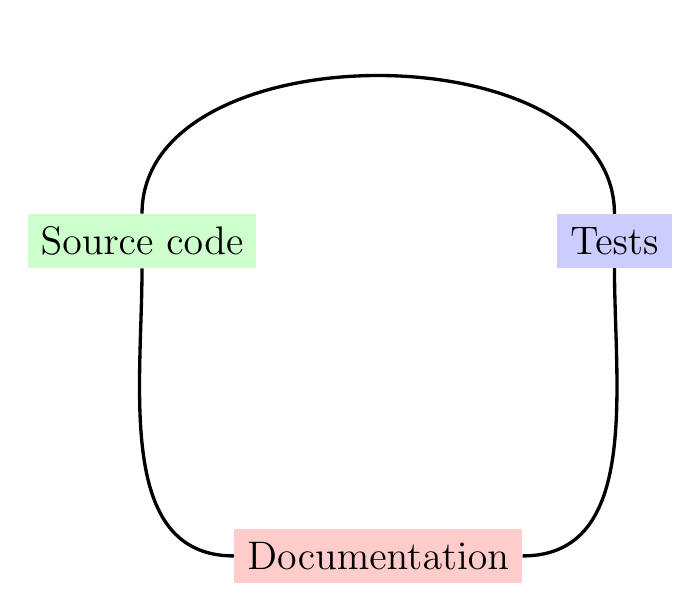
\begin{tikzpicture}
                \Large
                \node [fill=red!20] (docs) at (0, 0) {Documentation};
                \node [fill=blue!20] (tests) at (3, 4) {Tests};
                \node [fill=green!20] (source) at (-3, 4) {Source code};

                \draw [very thick] (docs) edge[out=0, in=-90] (tests);
                \draw [very thick] (tests) edge[out=90, in=90] (source);
                \draw [very thick] (source) edge[out=-90, in=180] (docs);
            \end{tikzpicture}
        \end{center}
    \end{frame}

    \begin{frame}
        \Huge
        \begin{center}
            Jupyter
        \end{center}
    \end{frame}


    \begin{frame}
        \begin{center}
            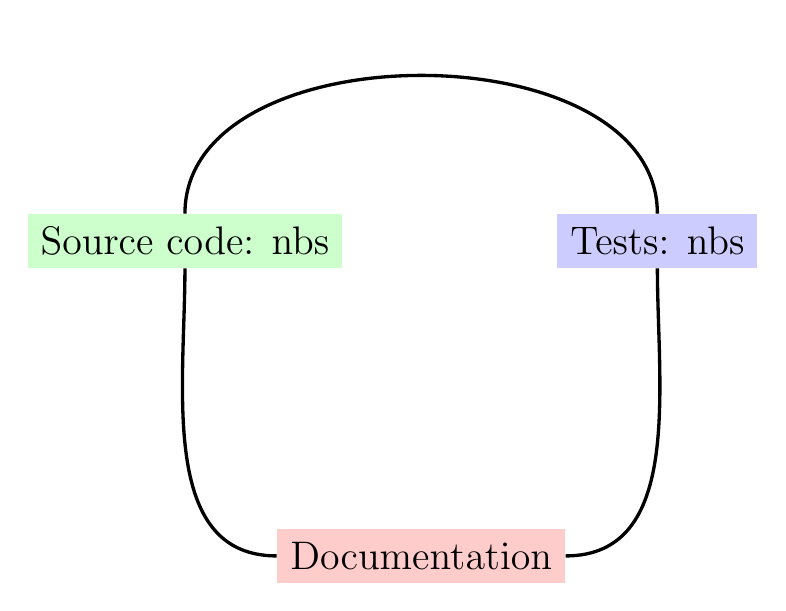
\begin{tikzpicture}
                \Large
                \node [fill=red!20] (docs) at (0, 0) {Documentation};
                \node [fill=blue!20] (tests) at (3, 4) {Tests: nbs};
                \node [fill=green!20] (source) at (-3, 4) {Source code: nbs};

                \draw [very thick] (docs) edge[out=0, in=-90] (tests);
                \draw [very thick] (tests) edge[out=90, in=90] (source);
                \draw [very thick] (source) edge[out=-90, in=180] (docs);
            \end{tikzpicture}
        \end{center}
    \end{frame}


    \begin{frame}
        \Large
        \begin{center}
            Research led teaching.
        \end{center}
    \end{frame}

    \begin{frame}
        \begin{center}
            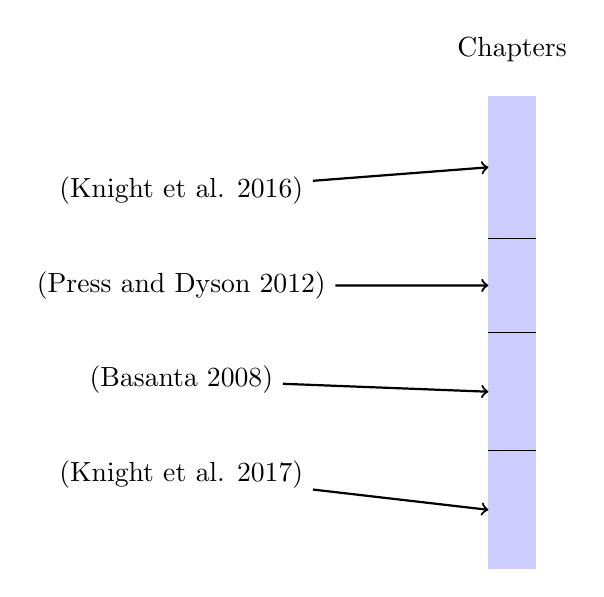
\begin{tikzpicture}[scale=0.6]
                \node (knight) at (0, 8) {(Knight et al. 2016)};
                \node (press) at ($(knight) + (0, -2)$) {(Press and Dyson 2012)};
                \node (basanta) at ($(press) + (0, -2)$) {(Basanta 2008)};
                \node (knight2017) at ($(basanta) + (0, -2)$) {(Knight et al.  2017)};

                \node at ($(knight) + (7, 3)$) {Chapters};

                \fill [blue!20] ($(knight) + (6.5, 2)$) rectangle ($(knight) + (7.5, -8)$);
                \draw ($(knight) + (6.5, -1)$) -- ($(knight) + (7.5, -1)$);
                \draw ($(knight) + (6.5, -3)$) -- ($(knight) + (7.5, -3)$);
                \draw ($(knight) + (6.5, -5.5)$) -- ($(knight) + (7.5, -5.5)$);

                \draw [thick, ->] (knight) -- ($(knight) + (6.5, .5)$);
                \draw [thick, ->] (press) -- ($(knight) + (6.5, -2)$);
                \draw [thick, ->] (basanta) -- ($(knight) + (6.5, -4.25)$);
                \draw [thick, ->] (knight2017) -- ($(knight) + (6.5, -6.75)$);
            \end{tikzpicture}
        \end{center}
    \end{frame}

    \begin{frame}
        \Huge
        \begin{center}
            Assessment
        \end{center}
    \end{frame}

    \begin{frame}
        \begin{itemize}
            \item Research software;
            \item Contemporary research.
        \end{itemize}
    \end{frame}

    \begin{frame}
        \begin{itemize}
            \item \url{https://github.com/Axelrod-Python/Axelrod}
            \item \url{https://github.com/drvinceknight/Nashpy}
            \item \url{https://github.com/drvinceknight/gt}
            \item \url{http://vknight.org/gt/}
        \end{itemize}
    \end{frame}

    \begin{frame}
        \begin{center}
            \includegraphics[width=.5\textwidth]{./static/Rutherford_Stephen_staff_profile.jpg}

            (Dr Stephen Rutherford. BIOSCI.)
        \end{center}
    \end{frame}

\end{document}
